\begin{figure}[t]
\begin{center}
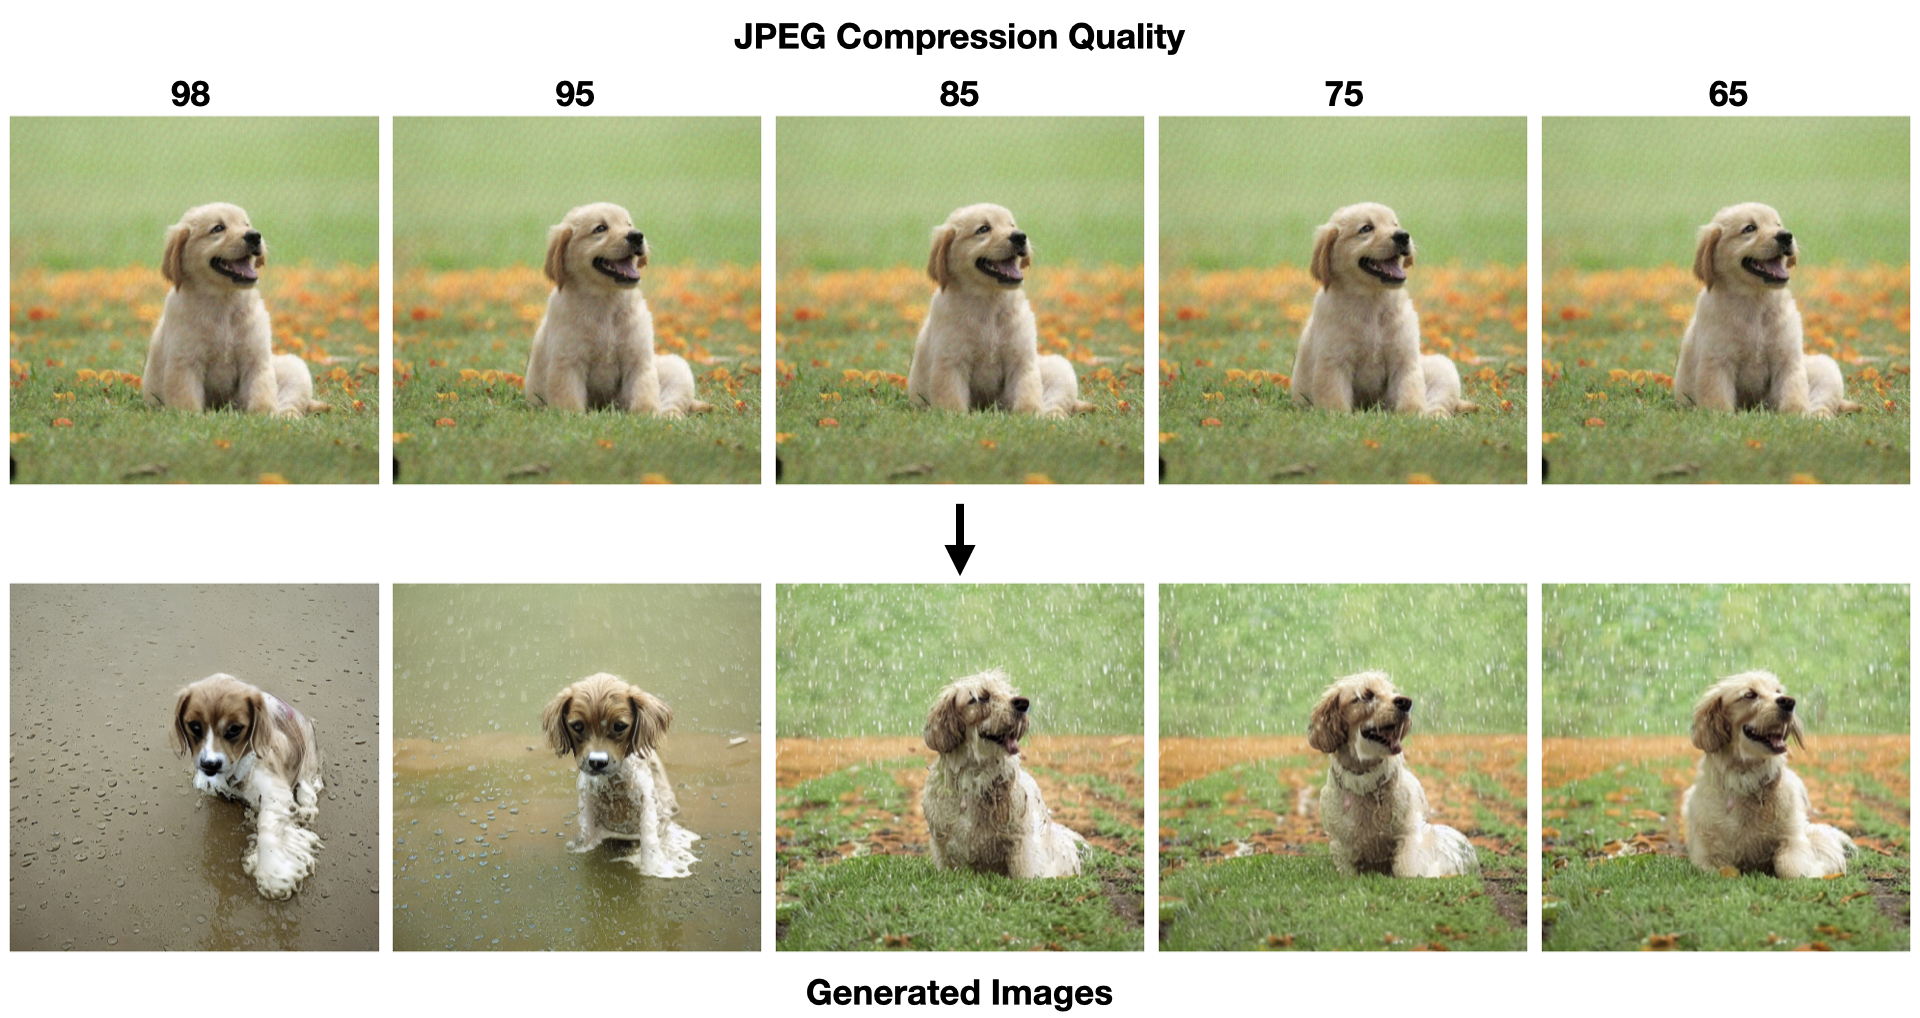
\includegraphics[width=0.75\textwidth]{images/jpeg-compression-figure.001.png}
\end{center}
\caption{\textbf{More JPEG compression more reliably undermines photoguard protection.} First row: We take a photoguard (Encoder attack) image  and JPEG compress it with varying quality. An image at 100\% JPEG quality is almost equivalent to the original photoguard image, while 65\% JPEG quality loses significant high-frequency information. Second row: Starting from the compressed image above, the adversary uses a diffusion model to make edits according to the same prompt setup as Figure~\ref{fig:img2img-overview}. With more compression, the generated content better maintains the original subject. Between compression quality of 95\% and 85\%, enough of the photoguard  noise is diminished, allowing stable image edits by an adversary.}
\label{figure-jpeg-compression-img2img}
\end{figure}